% EF5342 Week 8 — Derivatives (Futures, Forwards, Options)
% Beamer conversion from week8_Derivatives.pptx (59 source slides -> 38 frames).
% Compile: pdflatex week8_Derivatives.tex
% Each frame carries a [src: ...] comment mapping back to source slides.
\documentclass[aspectratio=169]{beamer}
\usepackage{../ef5342}
\usepackage{tikz}

\title{EF5342 Financial Systems, Markets and Instruments}
\subtitle{Week 8 --- Derivatives}
\author{Prof.\ Weikai Li}
\institute{City University of Hong Kong}
\date{Semester B 2026--2027}

\begin{document}

% [src: 1]
\begin{frame}
\titlepage
% Source slide 1 title image (slide01_img.jpg) dropped: decorative cover art.
\end{frame}

% [src: 2]
\section{Overview of Derivatives}
% Roadmap (source slide 2): Overview of Derivatives; Futures and Forwards;
% Options; Hedging and Speculation with Derivatives.

% [src: 3, 4]
\begin{frame}{What Are Derivatives, and Why Trade Them?}
\textbf{Derivatives} are securities whose value is derived from an underlying asset or financial instrument --- a stock, T-bill/bond, foreign currency, commodity, or even another derivative. They generally involve an agreement between two parties to exchange a quantity of an asset or cash flow at a predetermined price at a specified future date. Main types: \textbf{forwards, futures, options, swaps}.
\vspace{0.3em}
\begin{description}
  \item[Speculate] Profit from expected price changes in the underlying; no position in the underlying asset
  \item[Hedge] Minimize or manage risk; hold a position in the underlying with the goal of offsetting its risk
  \item[Arbitrage] Exploit price discrepancies between the underlying and its derivatives (e.g., covered interest rate parity arbitrage); simultaneous positions in both
\end{description}
\vspace{0.3em}
A derivative contract is a \textbf{zero-sum game}: what you gain, your counterparty loses.
\end{frame}

% [src: 5, 6]
\begin{frame}{Forwards vs.\ Futures}
\begin{description}
  \item[Spot contract] Agreement to transact involving the immediate exchange of assets and cash
  \item[Forward contract] Non-standardized agreement to buy or sell an asset in the future, with terms set today: customized, not traded in a secondary market (participants must perform), with \textbf{counterparty risk}
  \item[Futures contract] Standardized, exchange-traded version of a forward
\end{description}
\vspace{0.3em}
Futures differ from forwards:
\begin{itemize}
  \item \textbf{Liquid} --- most traders close out before delivery, so delivery may never take place
  \item \textbf{Marked to market daily} --- gains and losses realized each day as futures prices change
  \item \textbf{Clearing house} stands behind all contracts --- minimal counterparty default risk
  \item \textbf{Margin requirements} --- a deposit ensuring the terms of the contract will be met
\end{itemize}
\vspace{0.3em}
\emph{Post-crisis reform:} since the 2009 G20 Pittsburgh commitment, standardized OTC derivatives (e.g., interest-rate and credit-default swaps) must also clear through central counterparties --- implemented via Dodd-Frank Title VII (2010) in the US and EMIR (2012) in Europe.
\end{frame}

% [src: 7]
\begin{frame}{Futures Contracts: Mechanics}
\begin{description}
  \item[Long position] Purchase of a futures contract
  \item[Short position] Sale of a futures contract
  \item[Open interest] Total number of futures contracts outstanding at the beginning of the day
  \item[Clearing house] The unit that oversees trading on the exchange and guarantees all trades --- buyer to every clearing-member seller, seller to every buyer
\end{description}
\begin{center}

\includegraphics[height=0.40\textheight,keepaspectratio]{figures/slide07_img.png}
\end{center}
\note{The role of the clearing house is to perform the obligations under the contract agreed between the two counterparties, removing the counterparty risk the parties had to each other and replacing it with counterparty risk to a highly regulated central counterparty that specializes in managing and mitigating counterparty risk.}
\end{frame}

% [src: 8, 9]
\begin{frame}{Underlyings and Settlement}
The underlying asset can be T-notes/bonds, currency, commodity, stock index, single stock, or bitcoin (spot bitcoin ETFs and listed options on them are now mainstream exchange-traded products). Settlement is of two kinds:
\begin{description}
  \item[Physical delivery] The actual underlying asset is delivered on the specified delivery date
  \item[Cash settlement] Counterparties net out the cash difference in the value of their positions; no asset is delivered at expiration
\end{description}
\begin{center}

\includegraphics[height=0.42\textheight,keepaspectratio]{figures/slide09_img.png}
\end{center}
\end{frame}

% [src: 10, 11]
\begin{frame}{Example Contracts from CME}
\textbf{Physically settled}: Light Sweet Crude Oil (WTI) futures ---
\href{http://www.cmegroup.com/trading/energy/crude-oil/light-sweet-crude_contract_specifications.html}{cmegroup.com}
\vspace{0.2em}

\textbf{Cash-settled}: E-mini Crude Oil futures ---
\href{http://www.cmegroup.com/trading/energy/crude-oil/emini-crude-oil_contract_specifications.html}{cmegroup.com}
\begin{columns}
\begin{column}{0.5\textwidth}
\centering

\includegraphics[width=\textwidth,height=0.52\textheight,keepaspectratio]{figures/slide10_img.png}
\end{column}
\begin{column}{0.5\textwidth}
\centering

\includegraphics[width=\textwidth,height=0.52\textheight,keepaspectratio]{figures/slide11_img.png}
\end{column}
\end{columns}
\end{frame}

% [src: 12, 13]
\begin{frame}{Long and Short Positions: Profits at Maturity}
\textbf{Long} --- commitment to \emph{purchase} the asset on the delivery date; \textbf{short} --- commitment to \emph{sell}. At maturity:
\begin{itemize}
  \item Profit to long $=$ spot price at maturity $-$ original futures price
  \item Profit to short $=$ original futures price $-$ spot price at maturity
\end{itemize}
\begin{center}
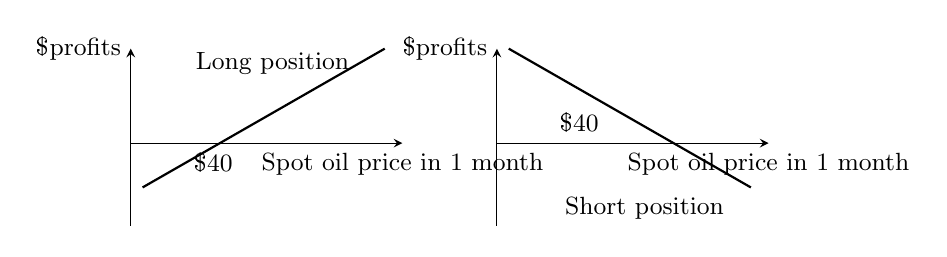
\begin{tikzpicture}[scale=0.75,>=stealth]
% Long position
\begin{scope}
\draw[->] (0,0) -- (4.6,0) node[below] {\small Spot oil price in 1 month};
\draw[->] (0,-1.4) -- (0,1.6) node[left] {\small \$profits};
\draw (1.4,0) node[below] {\small \$40};
\draw[thick] (0.2,-0.75) -- (4.3,1.6);
\node at (2.4,1.35) {\small Long position};
\end{scope}
\begin{scope}[xshift=6.2cm]
\draw[->] (0,0) -- (4.6,0) node[below] {\small Spot oil price in 1 month};
\draw[->] (0,-1.4) -- (0,1.6) node[left] {\small \$profits};
\draw (1.4,0) node[above] {\small \$40};
\draw[thick] (0.2,1.6) -- (4.3,-0.75);
\node at (2.5,-1.1) {\small Short position};
\end{scope}
\end{tikzpicture}
\end{center}
Long and short profit from opposite price movements; the futures contract is a zero-sum game --- gains and losses net out to zero. \textbf{You must know how to plot profits of a derivative at maturity} (horizontal axis: spot price of the underlying at maturity).
\end{frame}

% [src: 14]
\begin{frame}{Margin Requirements on Futures}
\begin{description}
  \item[Initial margin] Deposit required on futures trades to ensure the terms of the contracts will be met
  \item[Maintenance margin] Margin a trader must maintain once a position is taken --- if losses push the account below it, the customer gets a \textbf{margin call} and must deposit funds to restore the \emph{initial} margin to keep the position open
\end{description}
\vspace{0.3em}
Brokers can close out a customer's position if margin is not maintained. Margin requirements are set by exchanges and vary across contracts (and over time).
\end{frame}

% [src: 15, 16]
\begin{frame}{Example: 30-Year Treasury Bond Futures (CBOT)}
\begin{table}
\centering
\footnotesize
\setlength{\tabcolsep}{3pt}
\begin{tabular}{p{0.09\textwidth}p{0.09\textwidth}p{0.1\textwidth}p{0.12\textwidth}p{0.33\textwidth}p{0.07\textwidth}p{0.07\textwidth}}
\toprule
\textbf{Contract} & \textbf{Exchange} & \textbf{Delivery Months} & \textbf{Contract Size} & \textbf{Deliverable Instrument} & \textbf{IMR} & \textbf{MMR} \\
\midrule
T-Bond & CBOT & M, J, S, D & \$100{,}000 face value & T-bonds maturing at least 15 years (and no more than 25 years) from the delivery date & \$4{,}070 & \$3{,}700 \\
\bottomrule
\end{tabular}
\end{table}
\vspace{0.2em}
Going \textbf{long} one June contract $=$ agreeing to buy \$100{,}000 face value of T-bonds at the original futures price at June expiry; going \textbf{short} $=$ agreeing to deliver the bonds and receive that price. Each investor posts the IMR of \$4{,}070 at initiation and must maintain the MMR of \$3{,}700 while the position is open.
\note{Margin requirements (``performance bonds'') as of September 2026, per CME Group for the 30-Year US Treasury Bond futures contract (ZB); CME recalculates margins under SPAN as volatility changes, so see the CME website for updates. Similar contracts may be available on other exchanges with slightly different terms. The contract calls for delivery of bonds with a 6\% yield, and a price adjustment is made if they are not 6\% yield.}
\end{frame}

% [src: 17]
\begin{frame}{Marking to Market: Example}
IMR \$4{,}070, MMR \$3{,}700. You buy one June contract at the opening price of 98'16 ($98+16/32 = 98.5$); Monday settles at 98'10 ($98.3125$), Tuesday closes at 97'00. What is in your margin account after Tuesday's settle?
\begin{table}
\centering
\small
\begin{tabular}{p{0.1\textwidth}p{0.1\textwidth}p{0.2\textwidth}p{0.19\textwidth}p{0.19\textwidth}}
\toprule
\textbf{Long} & \textbf{Settle} & \textbf{Underlying Value} & \textbf{Price Change} & \textbf{Margin Account} \\
\midrule
Open & --- & \$98{,}500.00 & --- & \$4{,}070.00 \\
Mon. & 98'10 & \$98{,}312.50 & ($-$\$187.50) & \$3{,}882.50 \\
Tues. & 97'00 & \$97{,}000.00 & ($-$\$1{,}312.50) & \$2{,}570.00 \\
\multicolumn{4}{l}{\emph{Margin call (below \$3{,}700): add cash}} & \$1{,}500.00 \\
\multicolumn{4}{l}{} & \$4{,}070.00 \\
\bottomrule
\end{tabular}
\end{table}
\emph{Who receives the money taken out of your margin account?} The counterparties who gain (via the clearing house).
\note{The futures price is effectively updated with daily marking to market. In this example the IMR is restored when there is a margin call.}
\end{frame}

% [src: 18, 19]
\begin{frame}{Valuation of Futures and the Parity Condition}
\begin{columns}
\begin{column}{0.5\textwidth}
\centering

\includegraphics[width=\textwidth,keepaspectratio]{figures/slide18_img_flat.png}
\end{column}
\begin{column}{0.5\textwidth}
\centering

\includegraphics[width=\textwidth,keepaspectratio]{figures/slide19_img_flat.png}
\end{column}
\end{columns}
\note{Convenience yield: benefits from holding the underlying asset, such as profiting from temporary shortages and the ability to keep a production process running.}
\end{frame}

% [src: 20]
\begin{frame}{Contango vs.\ Backwardation}
\begin{columns}
\begin{column}{0.5\textwidth}
\centering

\includegraphics[width=\textwidth,keepaspectratio]{figures/slide20_img_flat.png}
\end{column}
\begin{column}{0.5\textwidth}
\centering
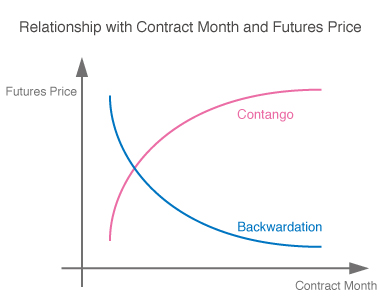
\includegraphics[width=\textwidth,keepaspectratio]{figures/slide20_img.jpg}
\end{column}
\end{columns}
\end{frame}

% [src: 21]
\begin{frame}{Basis}
Basis $=$ spot price $-$ futures price. The two converge as maturity approaches.
\begin{center}

\includegraphics[height=0.58\textheight,keepaspectratio]{figures/slide21_img_flat.png}
\end{center}
\end{frame}

% [src: 22]
\begin{frame}{Arbitrage with Futures}
Riskless profit is possible when the actual futures price differs from the price implied by the futures parity condition.
\vspace{0.3em}

\emph{Example.} Gold costs 2\% p.a.\ to store; the interest rate is 4\% p.a.; spot gold is \$4{,}000/oz (Sep 2026). The one-year futures price should be
\begin{equation*}
F = 4000 \times (1 + 0.02 + 0.04) = \$4{,}240
\end{equation*}
If the actual futures price is too high, e.g., \$4{,}250: borrow \$4{,}000, buy spot gold now (store for one year), and enter a futures contract to sell gold at \$4{,}250 in one year:
\begin{equation*}
\text{Profit (at maturity)} = -\$4000 \times (1+2\%+4\%) + \$4250 = \$10
\end{equation*}
\textbf{Question:} what if the actual futures price is too low, e.g., \$4{,}220?
\end{frame}

% [src: 23]
\begin{frame}{Risks of Trading Futures}
\begin{description}
  \item[Market risk] Speculators win or lose on price changes; hedgers hold the underlying and are unaffected by contract price volatility --- unless they cannot meet margin calls before expiration
  \item[Basis risk] Imperfect correlation between \% changes in futures and spot prices over the hedging period, producing an imperfect hedge (e.g., airlines hedging jet fuel with crude oil futures)
  \item[Liquidity risk] Thinly traded contracts make it hard to find a counterparty to close a position before maturity
  \item[Counterparty risk] High for forwards (default by the other party can cause large losses); mitigated in futures by daily marking to market and the clearing-house guarantee
\end{description}
\end{frame}

% [src: 24]
\section{Options}

% [src: 25, 26]
\begin{frame}{Options: Rights, Not Obligations}
Options give the buyer the \textbf{right but not the obligation} to buy or sell the underlying at a pre-specified price (the \textbf{strike price}) within a specific period. The buyer pays the seller a \textbf{premium}.
\begin{itemize}
  \item \textbf{Call} = right to buy; \textbf{put} = right to sell
  \item The \textbf{writer} (seller) receives the premium upfront and is \emph{obliged} to sell (call) or buy (put) if the buyer exercises
  \item Unlike futures/forwards: the option costs a premium, and the buyer can ``walk away'' --- losing only the premium
  \item \textbf{European} options: exercisable only at maturity; \textbf{American}: anytime up to maturity (most equity options are American)
\end{itemize}
\vspace{0.2em}
\textbf{Moneyness:} spot $=$ strike $\to$ ``at the money.'' \emph{In the money}: exercising immediately is profitable --- calls when $S > X$; puts when $S < X$. \emph{Out of the money}: the reverse.
\end{frame}

% [src: 27, 28]
\begin{frame}{Speculating with Call Options}
\textbf{Buy a call} when you think the spot price will rise above strike $X$: pay the premium for the right, but not the obligation, to buy at $X$.
\begin{itemize}
  \item $S > X$ at maturity: in the money --- exercise. Net profit $=$ spot at maturity $-$ strike $-$ premium
  \item $S \le X$: out of the money --- do not exercise; lose only the premium
\end{itemize}
\begin{center}
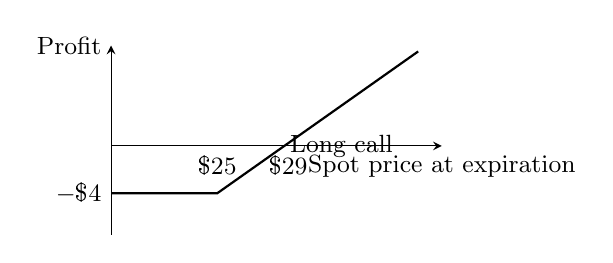
\begin{tikzpicture}[scale=0.75,>=stealth]
\draw[->] (0,0) -- (5.6,0) node[below] {\small Spot price at expiration};
\draw[->] (0,-1.5) -- (0,1.7) node[left] {\small Profit};
\draw (1.8,0) node[below] {\small \$25};
\draw (3.0,0) node[below] {\small \$29};
\draw (0,-0.8) node[left] {\small $-$\$4};
\draw[thick] (0,-0.8) -- (1.8,-0.8) -- (5.2,1.6);
\node at (3.9,0.0) {\small Long call};
\end{tikzpicture}
\end{center}
Long 1 call with strike \$25, premium \$4: loss capped at $-$\$4; break-even at \$29; unlimited upside.
\end{frame}

% [src: 29, 30]
\begin{frame}{Speculating with Put Options}
\textbf{Buy a put} when you think the spot price will fall below strike $X$: pay the premium for the right, but not the obligation, to sell at $X$.
\begin{itemize}
  \item $S < X$ at maturity: in the money --- exercise. Net profit $=$ strike $-$ spot at maturity $-$ premium
  \item $S \ge X$: out of the money --- do not exercise; lose only the premium
\end{itemize}
\begin{center}
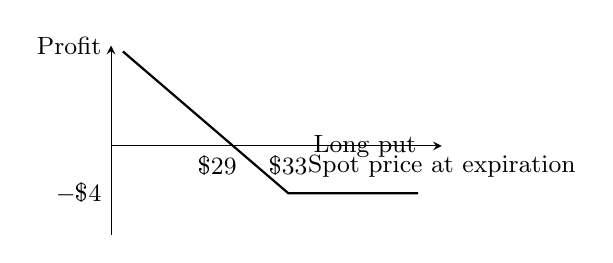
\begin{tikzpicture}[scale=0.75,>=stealth]
\draw[->] (0,0) -- (5.6,0) node[below] {\small Spot price at expiration};
\draw[->] (0,-1.5) -- (0,1.7) node[left] {\small Profit};
\draw (3.0,0) node[below] {\small \$33};
\draw (1.8,0) node[below] {\small \$29};
\draw (0,-0.8) node[left] {\small $-$\$4};
\draw[thick] (0.2,1.6) -- (3.0,-0.8) -- (5.2,-0.8);
\node at (4.3,0.0) {\small Long put};
\end{tikzpicture}
\end{center}
Long 1 put with strike \$33, premium \$4: loss capped at $-$\$4; break-even at \$29; maximum gain \$29 (if the spot goes to zero).
\end{frame}

% [src: 31]
\begin{frame}{Option Profit Profiles (All Four Positions)}
At maturity, with strike price $X$, call premium $c$, put premium $p$:
\begin{description}
  \item[Long call] Loss limited to $-c$ for $S_T \le X$, then $+$1-for-1 upside --- unlimited gain potential
  \item[Short call] Gain limited to $+c$ for $S_T \le X$, then $-$1-for-1 --- unlimited loss potential
  \item[Long put] Gain up to $X-p$ (when $S_T = 0$), loss limited to $-p$ for $S_T \ge X$
  \item[Short put] Loss up to $-(X-p)$ (when $S_T = 0$), gain limited to $+p$ for $S_T \ge X$
\end{description}
\vspace{0.3em}
All four are kinked at the strike price; buyers' losses are limited to the premium, writers' gains are limited to the premium.
\end{frame}

% [src: 32, 33]
\begin{frame}{Intrinsic Value and Time Value}
The option premium has an \textbf{intrinsic} and an \textbf{extrinsic} component:
\begin{itemize}
  \item Intrinsic value: calls $\max\{0, S-X\}$; puts $\max\{0, X-S\}$ ($X$ = strike, $S$ = spot) --- determined by moneyness
  \item Time value $=$ premium $-$ intrinsic value: the option has time value because the intrinsic value could still increase before maturity; it depends on volatility of the underlying, time to maturity, dividend yield, and interest rates
\end{itemize}
\begin{center}
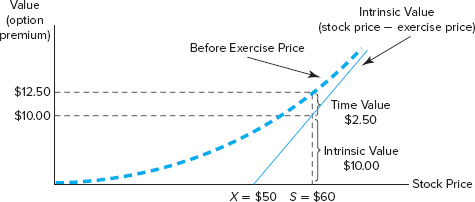
\includegraphics[height=0.40\textheight,keepaspectratio]{figures/slide33_img.jpg}
\end{center}
\begin{center}
\small Figure 10--9: The intrinsic value versus the before-exercise value of a call option
\end{center}
\end{frame}

% [src: 34]
\begin{frame}{Intrinsic and Time Value: Example}
\begin{table}
\centering
\footnotesize
\setlength{\tabcolsep}{3pt}
\begin{tabular}{p{0.12\textwidth}p{0.1\textwidth}p{0.1\textwidth}p{0.2\textwidth}p{0.1\textwidth}}
\toprule
\multicolumn{5}{l}{\textbf{MSFT} --- underlying stock price \$460.00; expiry Sep 18, 2026} \\
\midrule
\textbf{Type} & \textbf{Strike} & \textbf{Last} & \textbf{Bid / Ask} & \textbf{IV} \\
\midrule
Call & 460 & 34.84 & 34.30 / 35.95 & 38.4\% \\
Put & 495 & 3.68 & 3.60 / 3.90 & 23.7\% \\
\bottomrule
\end{tabular}
\end{table}
\vspace{0.2em}
With MSFT trading at \$460, the Sep \$460-strike call is \emph{at the money}: intrinsic value $= \max\{0,\, 460 - 460\} = \$0$, so its entire \$34.84 premium is \emph{time value}. Puts work the mirror way: a put is in the money only when $S < X$ --- the right to sell above \$460 is what would make a put strike such as \$495 valuable. Note the bid--ask spread: buyers pay the ask (\$35.95), sellers receive the bid (\$34.30) --- the spread is a round-trip trading cost.
\note{An investor would not exercise an American call early near expiry --- that would throw away the time value, which here is the entire premium. Aggregate open interest on this expiry is roughly 230{,}000 calls vs 130{,}000 puts, a mildly bullish tilt.}
\end{frame}

% [src: 35, 36]
\begin{frame}{Determinants of Option Prices}
Black and Scholes (1973) derived the formula for pricing an option from observable factors. Directional effects on the \emph{total} premium (intrinsic + extrinsic):
\begin{center}
\small
\begin{tabular}{p{0.5\textwidth}p{0.12\textwidth}p{0.12\textwidth}}
\toprule
\textbf{Factor} & \textbf{Call} & \textbf{Put} \\
\midrule
Current price of underlying & $+$ & $-$ \\
Strike price & $-$ & $+$ \\
Yield from holding underlying asset (div) & $-$ & $+$ \\
Time to maturity & $+$ & $+$ \\
Price volatility of underlying asset & $+$ & $+$ \\
Interest rate & $+$ & $-$ \\
\bottomrule
\end{tabular}
\end{center}
\vspace{0.1em}
\emph{Reasoning:} longer maturity $\Rightarrow$ more chance of getting in the money (both). Higher volatility $\Rightarrow$ options profit from favorable moves while downside is limited (both). Higher interest rates make calls more valuable (defer paying the spot price; invest at the high rate) and puts less valuable (the PV of the strike falls). Expected dividends push the stock price down on the ex-date while the strike is fixed $\Rightarrow$ calls less, puts more likely in the money.
\note{The higher the spot price, the more likely the call gets in the money; the higher the strike price, the less likely the call gets in the money.}
\end{frame}

% [src: 37, 38]
\begin{frame}{Volatility Indices: VIX and MOVE}
Option prices can be used to back out investors' expectations of market volatility (\textbf{implied volatility} --- forward-looking).
\begin{columns}
\begin{column}{0.5\textwidth}
\centering
\textbf{The VIX}: real-time index of market expectations for S\&P 500 volatility over the next 30 days --- the ``fear gauge,'' rising sharply during market stress. As of early September 2026 it sits near 14.5, versus a 12-month range of 13.4--35.3 (the high came with the March 2026 Iran-conflict spike).
\vspace{0.3em}


\includegraphics[width=0.88\textwidth,height=0.44\textheight,keepaspectratio]{figures/slide37_img_flat.png}
\end{column}
\begin{column}{0.5\textwidth}
\centering
\textbf{ICE BofA MOVE Index}: the bond market's ``VIX for bonds'' --- implied interest-rate volatility across U.S.\ Treasury markets; it can \emph{lead} equity volatility, sometimes signaling stress before the VIX. In late summer 2026 it trades near 74, within a trailing 12-month range of 40.7--108.8.
\vspace{0.3em}


\includegraphics[width=0.88\textwidth,height=0.44\textheight,keepaspectratio]{figures/slide38_img_flat.png}
\end{column}
\end{columns}
\end{frame}

% [src: 39]
\section{Hedging and Speculation with Derivatives}

% [src: 40, 41]
\begin{frame}{Hedging: First, Are You Long or Short the Underlying?}
Derivatives let investors and firms remove (hedge away) risks they do not want --- with futures/forwards or with options. To hedge, \textbf{take the opposite of your underlying spot position} in a futures/forward contract. So: is your underlying position long or short?
\vspace{0.3em}

\textbf{General rule:} you are \textbf{LONG} ``something'' (currency, stock, real estate, commodity) if you are happy when its price goes \textbf{up}; \textbf{SHORT} if you are happy when it goes \textbf{down}. Especially useful for natural positions from business or expected future actions:
\begin{itemize}
  \item You own a car --- long or short oil?
  \item You will buy an apartment in HK next year --- long or short HK real estate?
  \item A farmer growing wheat --- long or short wheat?
\end{itemize}
\note{Answers: car owner --- short oil; future apartment buyer --- short HK real estate (and short the funding, e.g., short Chinese Yuan in the original example); wheat farmer --- long wheat.}
\end{frame}

% [src: 42, 43]
\begin{frame}{Hedging with Futures: Example}
An investor must sell a stock in six months to fund a house down-payment. The stock is worth \$50 now; his profit/loss over the next six months is uncertain. \textbf{His underlying position is long the stock.}
\vspace{0.3em}

\textbf{Futures hedge:} short a futures contract on the stock. Assume the futures price is exactly \$50 (theoretical futures price: $F = S(1+r-d)$).
\begin{itemize}
  \item If the stock rises, he gains on the underlying but loses on the short futures --- gives up the upside
  \item If the stock falls, he loses on the underlying but gains on the short futures --- sheltered from the downside
  \item The hedge \textbf{completely eliminates} price risk of the underlying: the hedged profit profile is a flat line at \$0 (relative to today's \$50 price)
\end{itemize}
\end{frame}

% [src: 44]
\begin{frame}{Result of the Futures Hedge}
Hedged position $=$ underlying (long stock, profit line through \$50) $+$ short futures (mirror image): the combined profit is a \textbf{flat line} --- locked in at the futures price of \$50.
\vspace{0.4em}

\textbf{What is the point? Why not just sell the stock now?}
\begin{itemize}
  \item May be unable to sell (restrictions, or the underlying position is only expected --- the house purchase is future)
  \item Transaction costs of selling and repurchasing can exceed the hedge
  \item Under the futures parity condition, the hedge is equivalent to selling --- same expected payoff
  \item Flexibility: futures positions can be adjusted far more easily than the spot position
\end{itemize}
\note{Four reasons: cannot sell (restriction or nature of the underlying position); costs; equivalence via the futures parity condition; flexibility --- adjusting futures is easier than adjusting spot.}
\end{frame}

% [src: 45]
\begin{frame}{Basis Risk in Futures Hedging}
The textbook hedge is almost too good to be true. In practice:
\begin{itemize}
  \item The asset being hedged may differ from the asset underlying the futures contract
  \item The exact date of the future purchase/sale may be uncertain
  \item The hedge may require closing the futures position before its delivery month
\end{itemize}
\vspace{0.2em}
These give rise to \textbf{basis risk}: the spot--futures spread may widen or narrow between initiation and liquidation of the hedge.
\vspace{0.2em}

\emph{Example:} if the investor had to sell in three months, with spot at \$45 and futures at \$47, the net amount received is $\$45 + (\$50 - \$47) = \$48$ --- less than the expected \$50.
\end{frame}

% [src: 46, 47]
\begin{frame}{Hedging with Options: Retain Some Upside}
Can the investor keep some upside while limiting downside? Yes --- with options. Buy a 6-month \textbf{put} with strike $K = \$50$, premium \$4:
\begin{table}
\centering
\small
\begin{tabular}{p{0.14\textwidth}p{0.17\textwidth}p{0.17\textwidth}p{0.25\textwidth}p{0.11\textwidth}}
\toprule
\textbf{Stock at maturity} & \textbf{Long stock profit} & \textbf{Exercise put? ($K{=}\$50$)} & \textbf{Option profit (incl.\ premium)} & \textbf{Total} \\
\midrule
30 & $-$20 & Y & $20-4$ & $-$4 \\
40 & $-$10 & Y & $10-4$ & $-$4 \\
50 & 0 & Indifferent & $-$4 & $-$4 \\
54 & $+$4 & N & $-$4 & 0 \\
60 & $+$10 & N & $-$4 & $+$6 \\
70 & $+$20 & N & $-$4 & $+$16 \\
\bottomrule
\end{tabular}
\end{table}
Worst case limited to $-$\$4 (the premium); upside retained beyond \$54.
\end{frame}

% [src: 48]
\begin{frame}{Hedging a Long Position with a Long Put}
Combined profile $=$ (1) underlying long stock $+$ (2) long put $=$ (3) options hedge:
\begin{itemize}
  \item For stock prices at maturity below \$50: the put pays off --- total profit flat at $-$\$4 (the put premium)
  \item For stock prices above \$50: the put expires worthless --- total profit rises one-for-one with the stock, shifted down by \$4, breaking even at \$54
  \item Compared with the futures hedge (a flat line at \$50), the options hedge \textbf{retains the upside} at the cost of the \$4 premium
\end{itemize}
\end{frame}

% [src: 49]
\begin{frame}{Using Options to Hedge the Underlying}
\begin{description}
  \item[Long asset, long put] Hedge a \emph{long} position with a long put (the previous example): downside limited at $-p$, upside retained
  \item[Short asset, long call] Hedge a \emph{short} position with a long call: losses on the short asset above $K$ are offset by the call; downside of the hedge limited at $-c$
\end{description}
\vspace{0.3em}
Assume option strike $=$ asset price $= K$, put premium $= p$, call premium $= c$. The two combined profiles are mirror images: each floors the worst case at the premium paid while leaving one side of the price movement open.
\note{Put-call parity (simplified): $S + P = C$ plus a bond position.}
\end{frame}

% [src: 50]
\begin{frame}{Speculating with Options}
Options are particularly suitable for speculators betting on \emph{sophisticated} views of future price movement. With futures/forwards you can only bet on a rise or a fall; with options you can bet on:
\begin{itemize}
  \item A \textbf{large} rise/drop in the price of the underlying security
  \item A \textbf{moderate} rise/drop in the price of the underlying security
  \item The price moving \textbf{a lot in either direction} (long volatility)
  \item The price changing \textbf{little in either direction} (short volatility)
\end{itemize}
\end{frame}

% [src: 51]
\begin{frame}{Bull Spread Using Calls}
Buy a call with strike price $K_1$ and sell a call with strike price $K_2 > K_1$: profit is capped above $K_2$ and floored at the net premium. \textbf{Belief:} the underlying's price will rise, but only moderately.
\begin{center}

\includegraphics[height=0.52\textheight,keepaspectratio]{figures/slide51_img_flat.png}
\end{center}
% Source slide 51 second image (slide51_img1.png) dropped: duplicate payoff diagram.
\end{frame}

% [src: 52]
\begin{frame}{Bear Spread Using Puts}
Buy a put with strike price $K_2$ and sell a put with strike price $K_1 < K_2$: profit is capped below $K_1$. \textbf{Belief:} the underlying's price will fall, but only moderately.
\begin{center}

\includegraphics[height=0.52\textheight,keepaspectratio]{figures/slide52_img_flat.png}
\end{center}
% Source slide 52 second image (slide52_img1.png) dropped: duplicate payoff diagram.
\end{frame}

% [src: 53, 54]
\begin{frame}{Collar and Straddle}
\begin{description}
  \item[Collar] An options strategy that brackets the value of an asset between two bounds: long the underlying, buy an out-of-the-money \textbf{put} to limit downside, fund it by writing an out-of-the-money \textbf{call} (also limiting upside). Net outlay for the options is approximately zero. (Madoff claimed to use this strategy.)
  \item[Straddle] Long call + long put at the \emph{same} strike and maturity --- a bet on volatility. To profit, the stock price must move by more than the cost of both options, in \emph{either} direction. The writer of a straddle bets the price will not move much. Nick Leeson's short straddle caused the collapse of Barings Bank in January 1995; a modern parallel is Archegos (2021), whose leveraged total-return-swap positions imploded for \$36 billion of bank losses --- founder Sung Kook (Bill) Hwang was sentenced to 18 years in November 2024.
\end{description}
\note{WSJ: \href{https://blogs.wsj.com/marketbeat/2008/12/16/madoffs-not-so-unique-options-strategy/}{Madoff's not-so-unique options strategy}.}
\end{frame}

% [src: 55]
\begin{frame}{Put-Call Parity}
The call-plus-bond portfolio must cost the same as the stock-plus-put portfolio:
\begin{equation*}
C + \frac{X}{(1+r)^T} = S + P
\end{equation*}
where $C$ and $P$ price a call and put with the same maturity $T$ and strike $X$. At maturity both portfolios yield the same payoff regardless of $S_T$:
\begin{itemize}
  \item If $S_T > X$: the call is exercised (left $\to$ stock); the put expires worthless (right $\to$ stock)
  \item If $S_T < X$: the call expires worthless (left $\to$ receive $X$ from the bond); the put is exercised, selling the stock at $X$ (right $\to$ $X$)
\end{itemize}
\begin{center}

\includegraphics[height=0.33\textheight,keepaspectratio]{figures/slide55_img_flat.png}
\end{center}
\end{frame}

% [src: 56, 57]
\begin{frame}{Violation of Put-Call Parity: Example}
$S = 110$, $C = 17$, $P = 5$, risk-free rate 4\%, maturity 1 year, $X = 104$:
\begin{equation*}
C + X/(1+r) = 17 + 100 \;>\; S + P = 110 + 5
\end{equation*}
The right side is cheaper: buy the stock and a put, sell the call, and borrow the PV of the strike ($\$104/1.04 = \$100$):
\begin{center}
\small
\begin{tabular}{p{0.26\textwidth}p{0.15\textwidth}p{0.23\textwidth}p{0.23\textwidth}}
\toprule
\textbf{Position} & \textbf{Immediate CF} & \textbf{CF in 1 yr, $S_T < 104$} & \textbf{CF in 1 yr, $S_T \ge 104$} \\
\midrule
Buy stock & $-$110 & $S_T$ & $S_T$ \\
Borrow \$104/1.04 = \$100 & $+$100 & $-$104 & $-$104 \\
Sell a call option & $+$17 & 0 & $-(S_T - 104)$ \\
Buy a put option & $-$5 & $104 - S_T$ & 0 \\
\midrule
\textbf{Total} & \textbf{$+$2} & \textbf{0} & \textbf{0} \\
\bottomrule
\end{tabular}
\end{center}
Riskless profit of \$2 regardless of the stock price at maturity.
% Source slide 56 equation image (slide56_img.emf) dropped: EMF not supported; content typeset above.
\end{frame}

% [src: 58]
\begin{frame}{Key Takeaways: Derivatives and Futures}
\begin{description}
  \item[Derivatives] Securities with value derived from an underlying asset (stock, currency, commodity); used for speculation, hedging, or arbitrage; zero-sum game
  \item[Forwards vs.\ futures] Forwards: customized, OTC, counterparty risk, settled at maturity. Futures: standardized, exchange-traded, marked to market daily, clearing-house guarantee, margin requirements
  \item[Futures payoffs] Long: profit $=$ spot $-$ futures price (unlimited upside); short: futures price $-$ spot (unlimited downside)
\end{description}
\end{frame}

% [src: 59]
\begin{frame}{Key Takeaways: Options and Hedging}
\begin{description}
  \item[Options] Rights, not obligations. Call: right to buy; put: right to sell. Buyer pays premium --- limited loss, unlimited gain; writer receives premium --- limited gain, unlimited loss. Premium driven by underlying price, strike, maturity, volatility, interest rates
  \item[Hedging] Futures: take the opposite position to the underlying exposure --- eliminates risk and upside. Options: long put protects a long asset; long call protects a short asset
  \item[Parity conditions] Put--call: $C + X/(1+r)^T = S + P$; futures: $F = S(1+r)$, with dividend yield $F = S(1+r-d)$
\end{description}
% Source slide 59 formula images (slide59_img.png, slide59_img1.png) dropped: equations typeset natively above.
\end{frame}

\end{document}
